% $Id: christophe.tex,v 1.1 2001-06-09 11:14:35 geuzaine Exp $

\documentclass[a4]{seminar}

\usepackage{slides}

\graphicspath{{.}{fig/}}

\begin{document}

\talk{CNRS Grenoble June 20, 2001}

% ---------------------------------------------------------------------------

\begin{slide}

\slidepagestyle{reduced}

\begin{center}
\bigtitle{Benefits of an open software environment for the modeling of
          coupled electromagnetic problems}\\
\bigskip\bigskip
\medtitle{Christophe Geuzaine}\\
\bigskip
\medtitle{Deptartment of Electrical Engineering}\\
\medtitle{Montefiore Institute B28, Sart Tilman Campus}\\
\medtitle{University of Li�ge}\\
\medtitle{B-4000 Li�ge (BELGIUM)}
\end{center}

\end{slide}

% ---------------------------------------------------------------------------
\part{Introduction}
% ---------------------------------------------------------------------------

\chapter{Coupled electromagnetic problems?}

\begin{slide}

Maxwell's equations, with...

\begin{slideitemize}
\item Electric and electronic \emph{circuit} coupling (Power electronic supplies)
\item \emph{Mechanical} coupling (force calculation, magnetostriction,
piezoelectricity, noise and vibrations)
\item \emph{Thermal} coupling (thermal losses, induction heating, dielectric heating)
\item \emph{Fluid} dynamics coupling (charged particules, magnetohydrodynamics)
\end{slideitemize}

\end{slide}

% ---------------------------------------------------------------------------

\chapter{Computational methods?}

\begin{slide}

\begin{slideitemize}
\item \emph{Analytic} models are difficult/impossible to apply to complex/coupled problems
\item Basic \emph{theory} of classic numerical methods (Finite differences, finite
volumes, finite elements, integral methods) is now well known, and future
developments don't change the fundamental principles anymore
\item \emph{Performance} (both floating point and visualization) of low end PCs is
exploding
\end{slideitemize}

\end{slide}

% ---------------------------------------------------------------------------

\chapter{Finite element method (FEM)}

\begin{slide}

\begin{slideitemize}
\item 1960s for mechanical problems (very large \emph{application range} since 1980s)
\item Strong \emph{mathematical foundations} (convergence, unicity)
\item Generalizations/reinterpretations (vanishing boundaries between FEM,
FDM, FVM, ...) call for a \emph{single sofware implementation}
\end{slideitemize}

But not a magic tool:
\begin{slideitemize}
\item Many conflicting/\emph{antinomic} issues (continuous
vs. discontinuous, conform vs. non conform meshes, implicit vs. explicit,
...)
\item Generality always has a price (\emph{efficiency} tradeoff)
\end{slideitemize}

\end{slide}

\begin{slide}

Double discretization:

1) geometry: mesh finite number of elementary elements which... tri, qua, ...

2) function spaces: finite dimension spaces, local support basis
   functions...

Weak formulation: ...

Galerkin if basis functions=test functions.

\end{slide}

\begin{slide}

Example: magnetostatics

...

\end{slide}

\begin{slide}

In practice?

\begin{slideitemize}
\item Geometry (CAD)
\item Mesh
\item Solver: our focus today - GetDP: next slides
\item Post-processing
\end{slideitemize}

\end{slide}

% ---------------------------------------------------------------------------

% $Id: getdp-basics.tex,v 1.1 2001-06-09 11:14:35 geuzaine Exp $

% ---------------------------------------------------------------------------

\chapter{}

\begin{slide}

\slidepagestyle{reduced}

\begin{center}
\bigtitle{A general software environment for the treatment of discrete problems}\\
\bigtitle{(GetDP)}\\
\bigskip\bigskip
\medtitle{Patrick Dular, Christophe Geuzaine}\\
\bigskip
\medtitle{Deptartment of Electrical Engineering}\\
\medtitle{Montefiore Institute B28, Sart Tilman Campus}\\
\medtitle{University of Li�ge}\\
\medtitle{B-4000 Li�ge (BELGIUM)}
\end{center}

\end{slide}

% ---------------------------------------------------------------------------
\part{GetDP}
% ---------------------------------------------------------------------------

\chapter{An environment open to various couplings}

\begin{slide}

Any coupling between 
\begin{slideitemize}
\item \emph{Physical} problems (electromagnetic, thermal, mechanical, ...)
\item \emph{Numerical} methods (finite element methods, integral methods, ...)
\item \emph{Geometries} (1D, 2D, 2D axi, 3D)
\item \emph{Time} states (static, harmonic, transient)
\end{slideitemize}

How?
\begin{slideitemize}
\item Clear \emph{mathematical} definitions/structure
\item Directly transcribed into 10 interdependent \emph{objects}
\end{slideitemize}

\end{slide}

% ---------------------------------------------------------------------------

\chapter{Definition of discrete problems}

\begin{slide}

\begin{slideitemize}
\item Copy of formal mathematical expression of problems 
\item ASCII \emph{Text} file (``\code{.pro} file'')
\end{slideitemize}

\begin{center}
\scalebox{0.54}{\begin{picture}(0,0)%
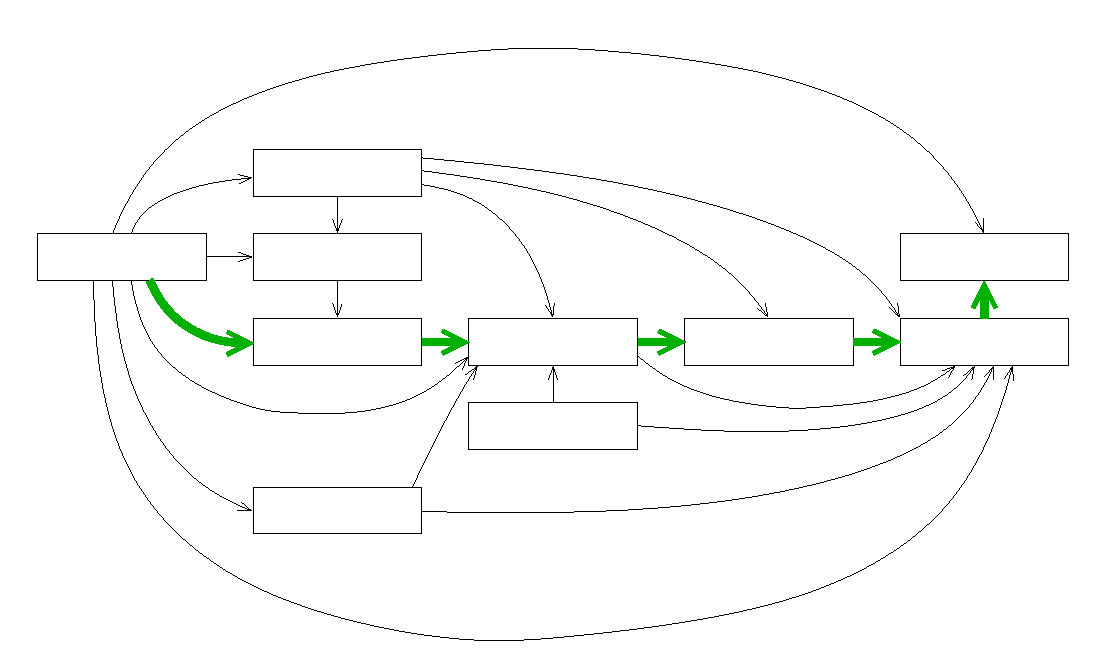
\includegraphics{getdp-struct}%
\end{picture}%
\setlength{\unitlength}{3947sp}%
%
\begingroup\makeatletter\ifx\SetFigFont\undefined%
\gdef\SetFigFont#1#2#3#4#5{%
  \reset@font\fontsize{#1}{#2pt}%
  \fontfamily{#3}\fontseries{#4}\fontshape{#5}%
  \selectfont}%
\fi\endgroup%
\begin{picture}(8552,4992)(300,-6402)
\put(1126,-3361){\makebox(0,0)[b]{\smash{\SetFigFont{10}{12.0}{\rmdefault}{\mddefault}{\updefault}{\color[rgb]{0,0,0}\code{Group}}%
}}}
\put(2851,-2686){\makebox(0,0)[b]{\smash{\SetFigFont{10}{12.0}{\rmdefault}{\mddefault}{\updefault}{\color[rgb]{0,0,0}\code{Function}}%
}}}
\put(2851,-3361){\makebox(0,0)[b]{\smash{\SetFigFont{10}{12.0}{\rmdefault}{\mddefault}{\updefault}{\color[rgb]{0,0,0}\code{Constraint}}%
}}}
\put(2851,-4036){\makebox(0,0)[b]{\smash{\SetFigFont{10}{12.0}{\rmdefault}{\mddefault}{\updefault}{\color[rgb]{0,0,0}\code{FunctionSpace}}%
}}}
\put(2851,-5386){\makebox(0,0)[b]{\smash{\SetFigFont{10}{12.0}{\rmdefault}{\mddefault}{\updefault}{\color[rgb]{0,0,0}\code{Jacobian}}%
}}}
\put(4576,-4711){\makebox(0,0)[b]{\smash{\SetFigFont{10}{12.0}{\rmdefault}{\mddefault}{\updefault}{\color[rgb]{0,0,0}\code{Integration}}%
}}}
\put(4576,-4036){\makebox(0,0)[b]{\smash{\SetFigFont{10}{12.0}{\rmdefault}{\mddefault}{\updefault}{\color[rgb]{0,0,0}\code{Formulation}}%
}}}
\put(6301,-4036){\makebox(0,0)[b]{\smash{\SetFigFont{10}{12.0}{\rmdefault}{\mddefault}{\updefault}{\color[rgb]{0,0,0}\code{Resolution}}%
}}}
\put(8026,-3361){\makebox(0,0)[b]{\smash{\SetFigFont{10}{12.0}{\rmdefault}{\mddefault}{\updefault}{\color[rgb]{0,0,0}\code{PostOperation}}%
}}}
\put(8026,-4036){\makebox(0,0)[b]{\smash{\SetFigFont{10}{12.0}{\rmdefault}{\mddefault}{\updefault}{\color[rgb]{0,0,0}\code{PostProcessing}}%
}}}
\end{picture}
}
\end{center}

\end{slide}

\begin{slide}

\begin{center}
Particular data of a problem\\
\medskip
\scalebox{0.54}{\begin{picture}(0,0)%
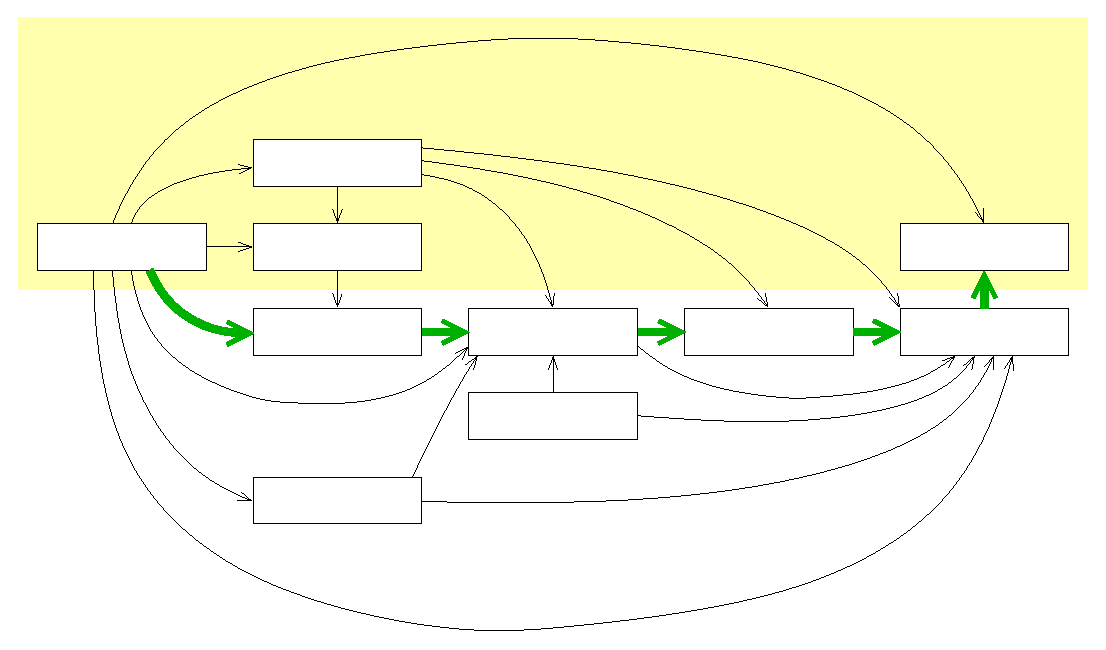
\includegraphics{getdp-struct-box}%
\end{picture}%
\setlength{\unitlength}{3947sp}%
%
\begingroup\makeatletter\ifx\SetFigFont\undefined%
\gdef\SetFigFont#1#2#3#4#5{%
  \reset@font\fontsize{#1}{#2pt}%
  \fontfamily{#3}\fontseries{#4}\fontshape{#5}%
  \selectfont}%
\fi\endgroup%
\begin{picture}(8552,4917)(300,-6402)
\put(1126,-3361){\makebox(0,0)[b]{\smash{\SetFigFont{10}{12.0}{\rmdefault}{\mddefault}{\updefault}{\color[rgb]{0,0,0}\code{Group}}%
}}}
\put(2851,-2686){\makebox(0,0)[b]{\smash{\SetFigFont{10}{12.0}{\rmdefault}{\mddefault}{\updefault}{\color[rgb]{0,0,0}\code{Function}}%
}}}
\put(2851,-3361){\makebox(0,0)[b]{\smash{\SetFigFont{10}{12.0}{\rmdefault}{\mddefault}{\updefault}{\color[rgb]{0,0,0}\code{Constraint}}%
}}}
\put(2851,-4036){\makebox(0,0)[b]{\smash{\SetFigFont{10}{12.0}{\rmdefault}{\mddefault}{\updefault}{\color[rgb]{0,0,0}\code{FunctionSpace}}%
}}}
\put(2851,-5386){\makebox(0,0)[b]{\smash{\SetFigFont{10}{12.0}{\rmdefault}{\mddefault}{\updefault}{\color[rgb]{0,0,0}\code{Jacobian}}%
}}}
\put(4576,-4711){\makebox(0,0)[b]{\smash{\SetFigFont{10}{12.0}{\rmdefault}{\mddefault}{\updefault}{\color[rgb]{0,0,0}\code{Integration}}%
}}}
\put(4576,-4036){\makebox(0,0)[b]{\smash{\SetFigFont{10}{12.0}{\rmdefault}{\mddefault}{\updefault}{\color[rgb]{0,0,0}\code{Formulation}}%
}}}
\put(6301,-4036){\makebox(0,0)[b]{\smash{\SetFigFont{10}{12.0}{\rmdefault}{\mddefault}{\updefault}{\color[rgb]{0,0,0}\code{Resolution}}%
}}}
\put(8026,-3361){\makebox(0,0)[b]{\smash{\SetFigFont{10}{12.0}{\rmdefault}{\mddefault}{\updefault}{\color[rgb]{0,0,0}\code{PostOperation}}%
}}}
\put(8026,-4036){\makebox(0,0)[b]{\smash{\SetFigFont{10}{12.0}{\rmdefault}{\mddefault}{\updefault}{\color[rgb]{0,0,0}\code{PostProcessing}}%
}}}
\end{picture}
}\\
\medskip
Method of resolution (``black box'')
\end{center}

\end{slide}

% ---------------------------------------------------------------------------

\background{7\semcm}{4.2\semcm}{\scalebox{0.3}{\begin{picture}(0,0)%
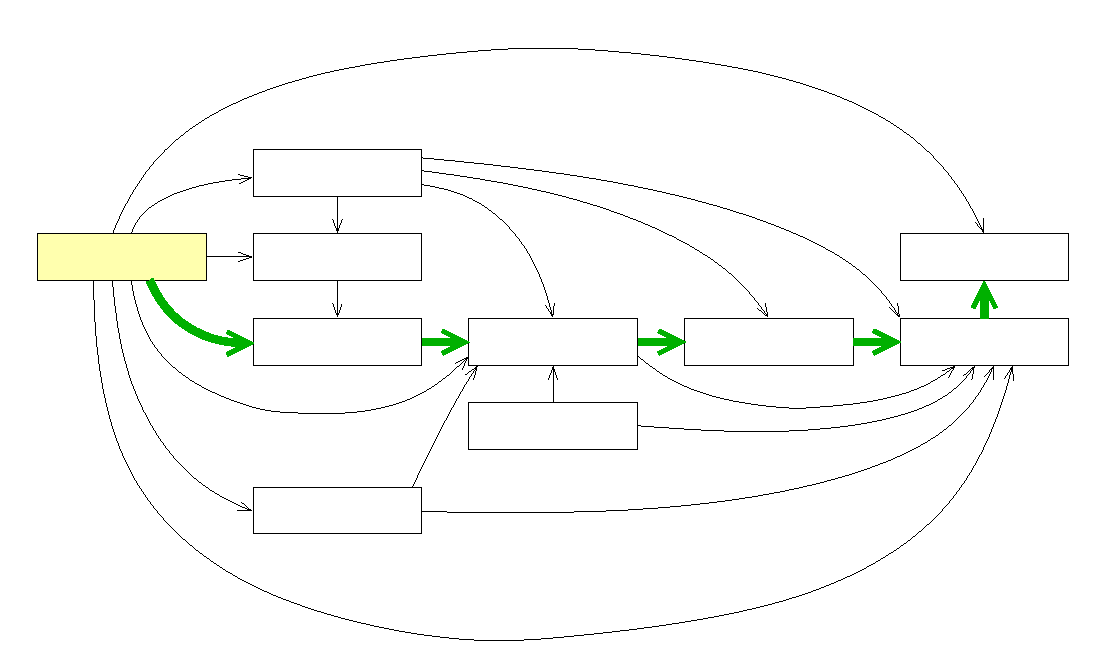
\includegraphics{getdp-struct-group}%
\end{picture}%
\setlength{\unitlength}{3947sp}%
%
\begingroup\makeatletter\ifx\SetFigFont\undefined%
\gdef\SetFigFont#1#2#3#4#5{%
  \reset@font\fontsize{#1}{#2pt}%
  \fontfamily{#3}\fontseries{#4}\fontshape{#5}%
  \selectfont}%
\fi\endgroup%
\begin{picture}(8274,4765)(439,-6402)
\put(1126,-3361){\makebox(0,0)[b]{\smash{\SetFigFont{10}{12.0}{\rmdefault}{\mddefault}{\updefault}{\color[rgb]{0,0,0}\code{Group}}%
}}}
\put(2851,-2686){\makebox(0,0)[b]{\smash{\SetFigFont{10}{12.0}{\rmdefault}{\mddefault}{\updefault}{\color[rgb]{0,0,0}\code{Function}}%
}}}
\put(2851,-3361){\makebox(0,0)[b]{\smash{\SetFigFont{10}{12.0}{\rmdefault}{\mddefault}{\updefault}{\color[rgb]{0,0,0}\code{Constraint}}%
}}}
\put(2851,-4036){\makebox(0,0)[b]{\smash{\SetFigFont{10}{12.0}{\rmdefault}{\mddefault}{\updefault}{\color[rgb]{0,0,0}\code{FunctionSpace}}%
}}}
\put(2851,-5386){\makebox(0,0)[b]{\smash{\SetFigFont{10}{12.0}{\rmdefault}{\mddefault}{\updefault}{\color[rgb]{0,0,0}\code{Jacobian}}%
}}}
\put(4576,-4711){\makebox(0,0)[b]{\smash{\SetFigFont{10}{12.0}{\rmdefault}{\mddefault}{\updefault}{\color[rgb]{0,0,0}\code{Integration}}%
}}}
\put(4576,-4036){\makebox(0,0)[b]{\smash{\SetFigFont{10}{12.0}{\rmdefault}{\mddefault}{\updefault}{\color[rgb]{0,0,0}\code{Formulation}}%
}}}
\put(6301,-4036){\makebox(0,0)[b]{\smash{\SetFigFont{10}{12.0}{\rmdefault}{\mddefault}{\updefault}{\color[rgb]{0,0,0}\code{Resolution}}%
}}}
\put(8026,-3361){\makebox(0,0)[b]{\smash{\SetFigFont{10}{12.0}{\rmdefault}{\mddefault}{\updefault}{\color[rgb]{0,0,0}\code{PostOperation}}%
}}}
\put(8026,-4036){\makebox(0,0)[b]{\smash{\SetFigFont{10}{12.0}{\rmdefault}{\mddefault}{\updefault}{\color[rgb]{0,0,0}\code{PostProcessing}}%
}}}
\end{picture}
}}

\chapter{\code{Group}: defining topological entities}

\begin{slide}

\mybox{colbox}{11\semcm}{
  \begin{slideitemize}
  \item Regions
  \item Functions on Regions (nodes, edges, edges of tree, ...)
  \end{slideitemize}
}

Example:

\begin{syntax}
Air = Region[1]; Core = Region[2];
    = ;
\end{syntax}



\end{slide}

% ---------------------------------------------------------------------------

\background{7\semcm}{4.2\semcm}{\scalebox{0.3}{\begin{picture}(0,0)%
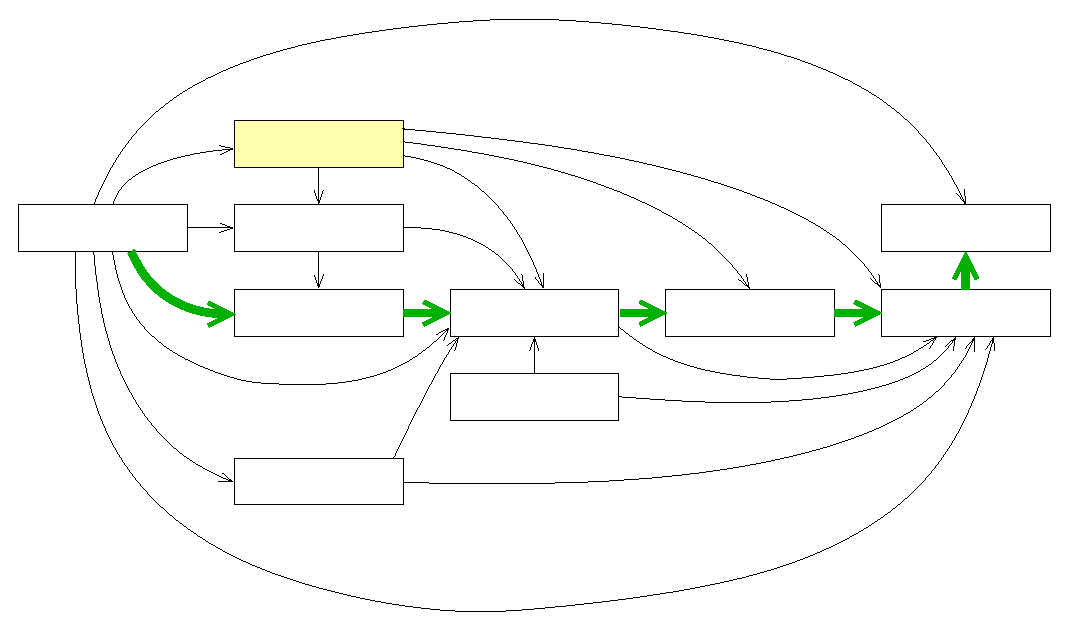
\includegraphics{getdp-struct-function}%
\end{picture}%
\setlength{\unitlength}{3947sp}%
%
\begingroup\makeatletter\ifx\SetFigFont\undefined%
\gdef\SetFigFont#1#2#3#4#5{%
  \reset@font\fontsize{#1}{#2pt}%
  \fontfamily{#3}\fontseries{#4}\fontshape{#5}%
  \selectfont}%
\fi\endgroup%
\begin{picture}(8274,4765)(439,-6402)
\put(1126,-3361){\makebox(0,0)[b]{\smash{\SetFigFont{10}{12.0}{\rmdefault}{\mddefault}{\updefault}{\color[rgb]{0,0,0}\code{Group}}%
}}}
\put(2851,-2686){\makebox(0,0)[b]{\smash{\SetFigFont{10}{12.0}{\rmdefault}{\mddefault}{\updefault}{\color[rgb]{0,0,0}\code{Function}}%
}}}
\put(2851,-3361){\makebox(0,0)[b]{\smash{\SetFigFont{10}{12.0}{\rmdefault}{\mddefault}{\updefault}{\color[rgb]{0,0,0}\code{Constraint}}%
}}}
\put(2851,-4036){\makebox(0,0)[b]{\smash{\SetFigFont{10}{12.0}{\rmdefault}{\mddefault}{\updefault}{\color[rgb]{0,0,0}\code{FunctionSpace}}%
}}}
\put(2851,-5386){\makebox(0,0)[b]{\smash{\SetFigFont{10}{12.0}{\rmdefault}{\mddefault}{\updefault}{\color[rgb]{0,0,0}\code{Jacobian}}%
}}}
\put(4576,-4711){\makebox(0,0)[b]{\smash{\SetFigFont{10}{12.0}{\rmdefault}{\mddefault}{\updefault}{\color[rgb]{0,0,0}\code{Integration}}%
}}}
\put(4576,-4036){\makebox(0,0)[b]{\smash{\SetFigFont{10}{12.0}{\rmdefault}{\mddefault}{\updefault}{\color[rgb]{0,0,0}\code{Formulation}}%
}}}
\put(6301,-4036){\makebox(0,0)[b]{\smash{\SetFigFont{10}{12.0}{\rmdefault}{\mddefault}{\updefault}{\color[rgb]{0,0,0}\code{Resolution}}%
}}}
\put(8026,-3361){\makebox(0,0)[b]{\smash{\SetFigFont{10}{12.0}{\rmdefault}{\mddefault}{\updefault}{\color[rgb]{0,0,0}\code{PostOperation}}%
}}}
\put(8026,-4036){\makebox(0,0)[b]{\smash{\SetFigFont{10}{12.0}{\rmdefault}{\mddefault}{\updefault}{\color[rgb]{0,0,0}\code{PostProcessing}}%
}}}
\end{picture}
}}

\chapter{\code{Function}: defining expressions}

\begin{slide}

\mybox{colbox}{11\semcm}{
  \begin{slideitemize}
  \item Physical characteristics
  \item Time functions
  \item Various other functions (natural contraints, ...)
  \end{slideitemize}
}

Example:


\end{slide}

% ---------------------------------------------------------------------------

\background{7\semcm}{4.2\semcm}{\scalebox{0.3}{\begin{picture}(0,0)%
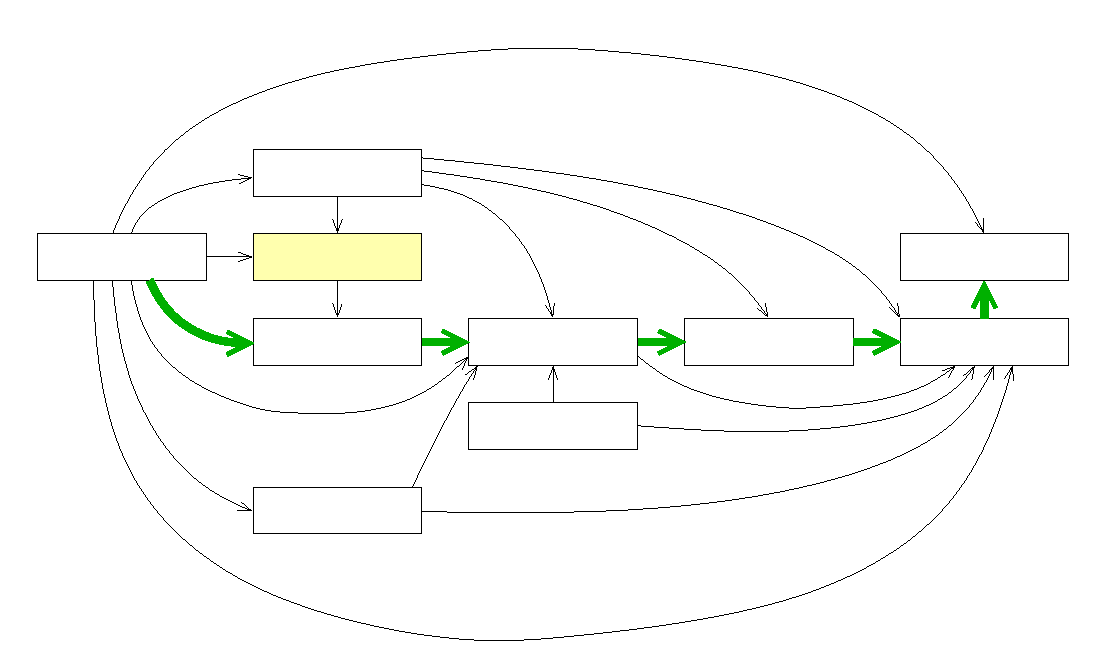
\includegraphics{getdp-struct-constraint}%
\end{picture}%
\setlength{\unitlength}{3947sp}%
%
\begingroup\makeatletter\ifx\SetFigFont\undefined%
\gdef\SetFigFont#1#2#3#4#5{%
  \reset@font\fontsize{#1}{#2pt}%
  \fontfamily{#3}\fontseries{#4}\fontshape{#5}%
  \selectfont}%
\fi\endgroup%
\begin{picture}(8274,4765)(439,-6402)
\put(1126,-3361){\makebox(0,0)[b]{\smash{\SetFigFont{10}{12.0}{\rmdefault}{\mddefault}{\updefault}{\color[rgb]{0,0,0}\code{Group}}%
}}}
\put(2851,-2686){\makebox(0,0)[b]{\smash{\SetFigFont{10}{12.0}{\rmdefault}{\mddefault}{\updefault}{\color[rgb]{0,0,0}\code{Function}}%
}}}
\put(2851,-3361){\makebox(0,0)[b]{\smash{\SetFigFont{10}{12.0}{\rmdefault}{\mddefault}{\updefault}{\color[rgb]{0,0,0}\code{Constraint}}%
}}}
\put(2851,-4036){\makebox(0,0)[b]{\smash{\SetFigFont{10}{12.0}{\rmdefault}{\mddefault}{\updefault}{\color[rgb]{0,0,0}\code{FunctionSpace}}%
}}}
\put(2851,-5386){\makebox(0,0)[b]{\smash{\SetFigFont{10}{12.0}{\rmdefault}{\mddefault}{\updefault}{\color[rgb]{0,0,0}\code{Jacobian}}%
}}}
\put(4576,-4711){\makebox(0,0)[b]{\smash{\SetFigFont{10}{12.0}{\rmdefault}{\mddefault}{\updefault}{\color[rgb]{0,0,0}\code{Integration}}%
}}}
\put(4576,-4036){\makebox(0,0)[b]{\smash{\SetFigFont{10}{12.0}{\rmdefault}{\mddefault}{\updefault}{\color[rgb]{0,0,0}\code{Formulation}}%
}}}
\put(6301,-4036){\makebox(0,0)[b]{\smash{\SetFigFont{10}{12.0}{\rmdefault}{\mddefault}{\updefault}{\color[rgb]{0,0,0}\code{Resolution}}%
}}}
\put(8026,-3361){\makebox(0,0)[b]{\smash{\SetFigFont{10}{12.0}{\rmdefault}{\mddefault}{\updefault}{\color[rgb]{0,0,0}\code{PostOperation}}%
}}}
\put(8026,-4036){\makebox(0,0)[b]{\smash{\SetFigFont{10}{12.0}{\rmdefault}{\mddefault}{\updefault}{\color[rgb]{0,0,0}\code{PostProcessing}}%
}}}
\end{picture}
}}

\chapter{\code{Constraint}: specifying constraints}

\begin{slide}

\mybox{colbox}{11\semcm}{
  \begin{slideitemize}
  \item Boundary conditions (classical, connection)
  \item Initial conditions
  \item Topology of circuits with lumped elements
  \item Other constraints (on local and global quantities)
  \end{slideitemize}
}

Example:


\end{slide}

% ---------------------------------------------------------------------------

\background{7\semcm}{4.2\semcm}{\scalebox{0.3}{\begin{picture}(0,0)%
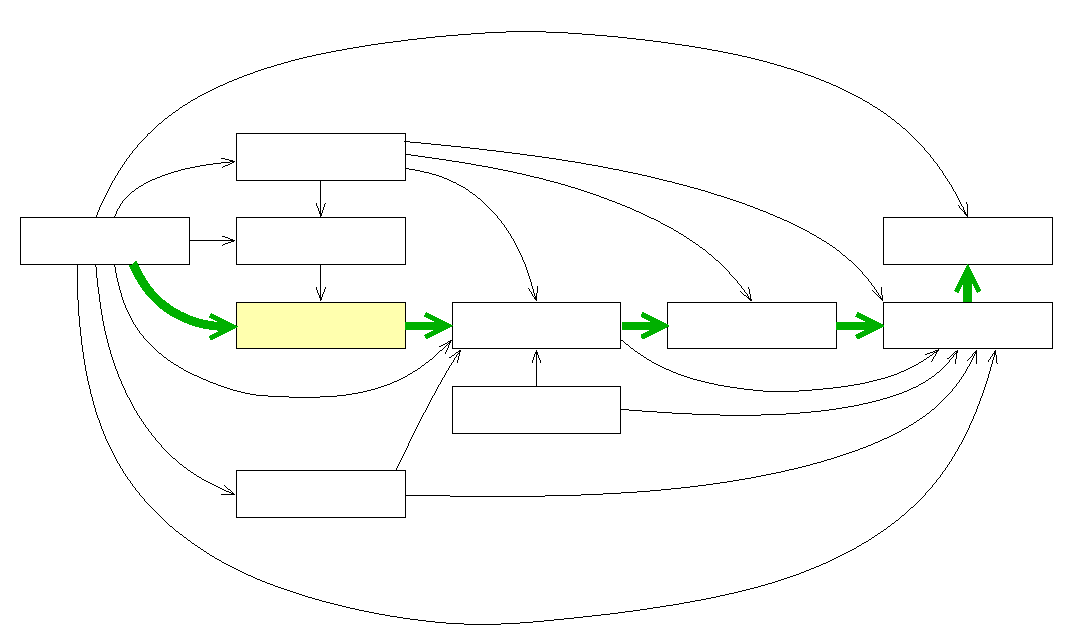
\includegraphics{getdp-struct-functionspace}%
\end{picture}%
\setlength{\unitlength}{3947sp}%
%
\begingroup\makeatletter\ifx\SetFigFont\undefined%
\gdef\SetFigFont#1#2#3#4#5{%
  \reset@font\fontsize{#1}{#2pt}%
  \fontfamily{#3}\fontseries{#4}\fontshape{#5}%
  \selectfont}%
\fi\endgroup%
\begin{picture}(8552,4992)(300,-6402)
\put(1126,-3361){\makebox(0,0)[b]{\smash{\SetFigFont{10}{12.0}{\rmdefault}{\mddefault}{\updefault}{\color[rgb]{0,0,0}\code{Group}}%
}}}
\put(2851,-2686){\makebox(0,0)[b]{\smash{\SetFigFont{10}{12.0}{\rmdefault}{\mddefault}{\updefault}{\color[rgb]{0,0,0}\code{Function}}%
}}}
\put(2851,-3361){\makebox(0,0)[b]{\smash{\SetFigFont{10}{12.0}{\rmdefault}{\mddefault}{\updefault}{\color[rgb]{0,0,0}\code{Constraint}}%
}}}
\put(2851,-4036){\makebox(0,0)[b]{\smash{\SetFigFont{10}{12.0}{\rmdefault}{\mddefault}{\updefault}{\color[rgb]{0,0,0}\code{FunctionSpace}}%
}}}
\put(2851,-5386){\makebox(0,0)[b]{\smash{\SetFigFont{10}{12.0}{\rmdefault}{\mddefault}{\updefault}{\color[rgb]{0,0,0}\code{Jacobian}}%
}}}
\put(4576,-4711){\makebox(0,0)[b]{\smash{\SetFigFont{10}{12.0}{\rmdefault}{\mddefault}{\updefault}{\color[rgb]{0,0,0}\code{Integration}}%
}}}
\put(4576,-4036){\makebox(0,0)[b]{\smash{\SetFigFont{10}{12.0}{\rmdefault}{\mddefault}{\updefault}{\color[rgb]{0,0,0}\code{Formulation}}%
}}}
\put(6301,-4036){\makebox(0,0)[b]{\smash{\SetFigFont{10}{12.0}{\rmdefault}{\mddefault}{\updefault}{\color[rgb]{0,0,0}\code{Resolution}}%
}}}
\put(8026,-3361){\makebox(0,0)[b]{\smash{\SetFigFont{10}{12.0}{\rmdefault}{\mddefault}{\updefault}{\color[rgb]{0,0,0}\code{PostOperation}}%
}}}
\put(8026,-4036){\makebox(0,0)[b]{\smash{\SetFigFont{10}{12.0}{\rmdefault}{\mddefault}{\updefault}{\color[rgb]{0,0,0}\code{PostProcessing}}%
}}}
\end{picture}
}}

\chapter{\code{FunctionSpace}: building function spaces}

\begin{slide}



Example:


\end{slide}

% ---------------------------------------------------------------------------

\background{7\semcm}{4.2\semcm}{\scalebox{0.3}{\begin{picture}(0,0)%
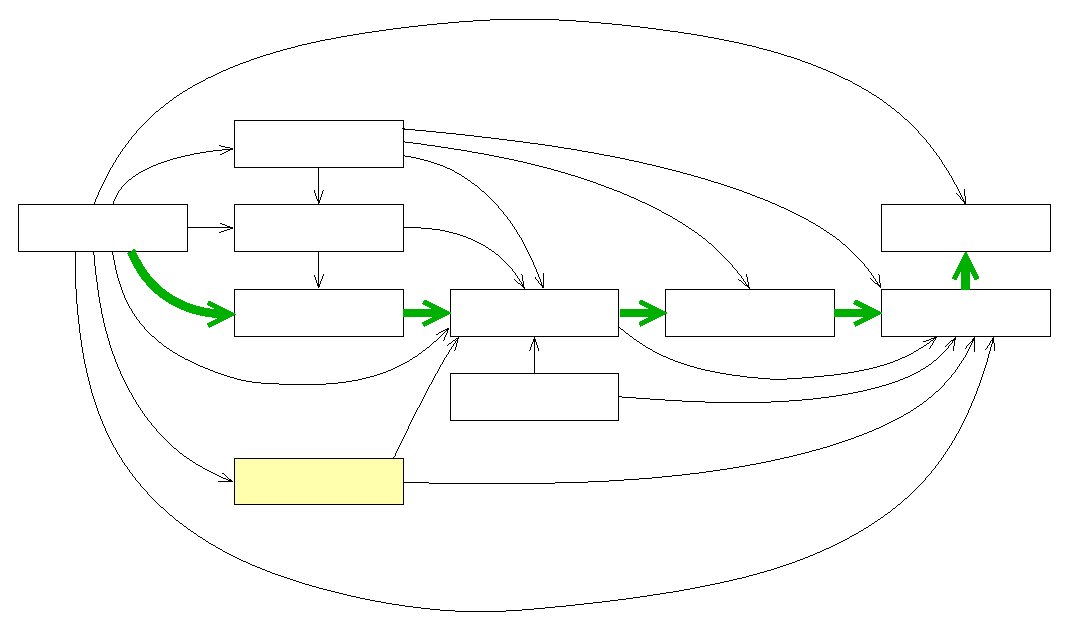
\includegraphics{getdp-struct-jacobian}%
\end{picture}%
\setlength{\unitlength}{3947sp}%
%
\begingroup\makeatletter\ifx\SetFigFont\undefined%
\gdef\SetFigFont#1#2#3#4#5{%
  \reset@font\fontsize{#1}{#2pt}%
  \fontfamily{#3}\fontseries{#4}\fontshape{#5}%
  \selectfont}%
\fi\endgroup%
\begin{picture}(8274,4765)(439,-6402)
\put(1126,-3361){\makebox(0,0)[b]{\smash{\SetFigFont{10}{12.0}{\rmdefault}{\mddefault}{\updefault}{\color[rgb]{0,0,0}\code{Group}}%
}}}
\put(2851,-2686){\makebox(0,0)[b]{\smash{\SetFigFont{10}{12.0}{\rmdefault}{\mddefault}{\updefault}{\color[rgb]{0,0,0}\code{Function}}%
}}}
\put(2851,-3361){\makebox(0,0)[b]{\smash{\SetFigFont{10}{12.0}{\rmdefault}{\mddefault}{\updefault}{\color[rgb]{0,0,0}\code{Constraint}}%
}}}
\put(2851,-4036){\makebox(0,0)[b]{\smash{\SetFigFont{10}{12.0}{\rmdefault}{\mddefault}{\updefault}{\color[rgb]{0,0,0}\code{FunctionSpace}}%
}}}
\put(2851,-5386){\makebox(0,0)[b]{\smash{\SetFigFont{10}{12.0}{\rmdefault}{\mddefault}{\updefault}{\color[rgb]{0,0,0}\code{Jacobian}}%
}}}
\put(4576,-4711){\makebox(0,0)[b]{\smash{\SetFigFont{10}{12.0}{\rmdefault}{\mddefault}{\updefault}{\color[rgb]{0,0,0}\code{Integration}}%
}}}
\put(4576,-4036){\makebox(0,0)[b]{\smash{\SetFigFont{10}{12.0}{\rmdefault}{\mddefault}{\updefault}{\color[rgb]{0,0,0}\code{Formulation}}%
}}}
\put(6301,-4036){\makebox(0,0)[b]{\smash{\SetFigFont{10}{12.0}{\rmdefault}{\mddefault}{\updefault}{\color[rgb]{0,0,0}\code{Resolution}}%
}}}
\put(8026,-3361){\makebox(0,0)[b]{\smash{\SetFigFont{10}{12.0}{\rmdefault}{\mddefault}{\updefault}{\color[rgb]{0,0,0}\code{PostOperation}}%
}}}
\put(8026,-4036){\makebox(0,0)[b]{\smash{\SetFigFont{10}{12.0}{\rmdefault}{\mddefault}{\updefault}{\color[rgb]{0,0,0}\code{PostProcessing}}%
}}}
\end{picture}
}}

\chapter{\code{Jacobian}: defining jacobian methods}

\begin{slide}


Example:


\end{slide}

% ---------------------------------------------------------------------------

\background{7\semcm}{4.2\semcm}{\scalebox{0.3}{\begin{picture}(0,0)%
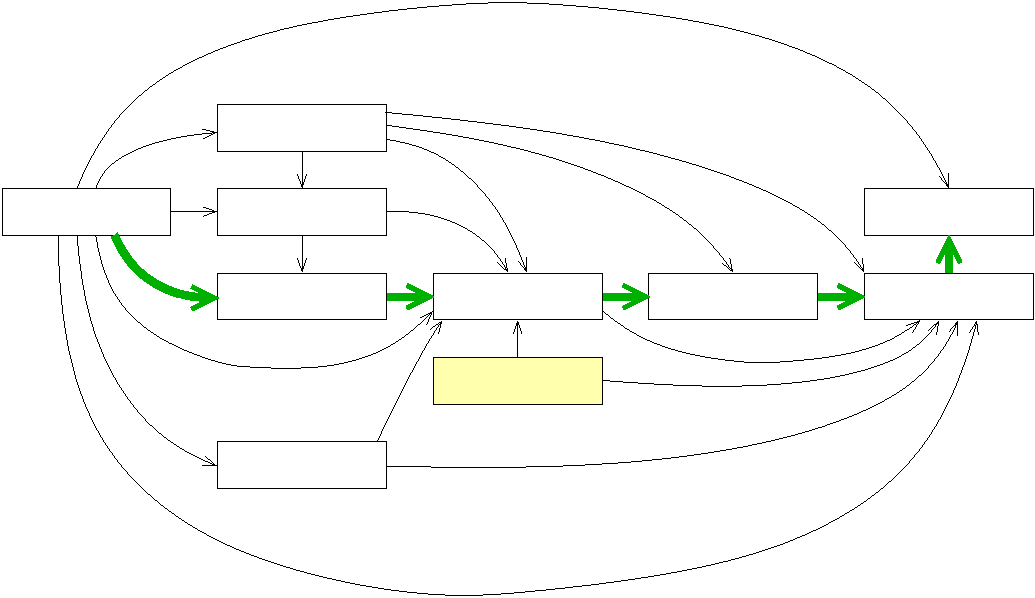
\includegraphics{getdp-struct-integration}%
\end{picture}%
\setlength{\unitlength}{3947sp}%
%
\begingroup\makeatletter\ifx\SetFigFont\undefined%
\gdef\SetFigFont#1#2#3#4#5{%
  \reset@font\fontsize{#1}{#2pt}%
  \fontfamily{#3}\fontseries{#4}\fontshape{#5}%
  \selectfont}%
\fi\endgroup%
\begin{picture}(8552,4992)(300,-6402)
\put(1126,-3361){\makebox(0,0)[b]{\smash{\SetFigFont{10}{12.0}{\rmdefault}{\mddefault}{\updefault}{\color[rgb]{0,0,0}\code{Group}}%
}}}
\put(2851,-2686){\makebox(0,0)[b]{\smash{\SetFigFont{10}{12.0}{\rmdefault}{\mddefault}{\updefault}{\color[rgb]{0,0,0}\code{Function}}%
}}}
\put(2851,-3361){\makebox(0,0)[b]{\smash{\SetFigFont{10}{12.0}{\rmdefault}{\mddefault}{\updefault}{\color[rgb]{0,0,0}\code{Constraint}}%
}}}
\put(2851,-4036){\makebox(0,0)[b]{\smash{\SetFigFont{10}{12.0}{\rmdefault}{\mddefault}{\updefault}{\color[rgb]{0,0,0}\code{FunctionSpace}}%
}}}
\put(2851,-5386){\makebox(0,0)[b]{\smash{\SetFigFont{10}{12.0}{\rmdefault}{\mddefault}{\updefault}{\color[rgb]{0,0,0}\code{Jacobian}}%
}}}
\put(4576,-4711){\makebox(0,0)[b]{\smash{\SetFigFont{10}{12.0}{\rmdefault}{\mddefault}{\updefault}{\color[rgb]{0,0,0}\code{Integration}}%
}}}
\put(4576,-4036){\makebox(0,0)[b]{\smash{\SetFigFont{10}{12.0}{\rmdefault}{\mddefault}{\updefault}{\color[rgb]{0,0,0}\code{Formulation}}%
}}}
\put(6301,-4036){\makebox(0,0)[b]{\smash{\SetFigFont{10}{12.0}{\rmdefault}{\mddefault}{\updefault}{\color[rgb]{0,0,0}\code{Resolution}}%
}}}
\put(8026,-3361){\makebox(0,0)[b]{\smash{\SetFigFont{10}{12.0}{\rmdefault}{\mddefault}{\updefault}{\color[rgb]{0,0,0}\code{PostOperation}}%
}}}
\put(8026,-4036){\makebox(0,0)[b]{\smash{\SetFigFont{10}{12.0}{\rmdefault}{\mddefault}{\updefault}{\color[rgb]{0,0,0}\code{PostProcessing}}%
}}}
\end{picture}
}}

\chapter{\code{Integration}: defining integration methods}

\begin{slide}



Example:


\end{slide}

% ---------------------------------------------------------------------------

\background{7\semcm}{4.2\semcm}{\scalebox{0.3}{\begin{picture}(0,0)%
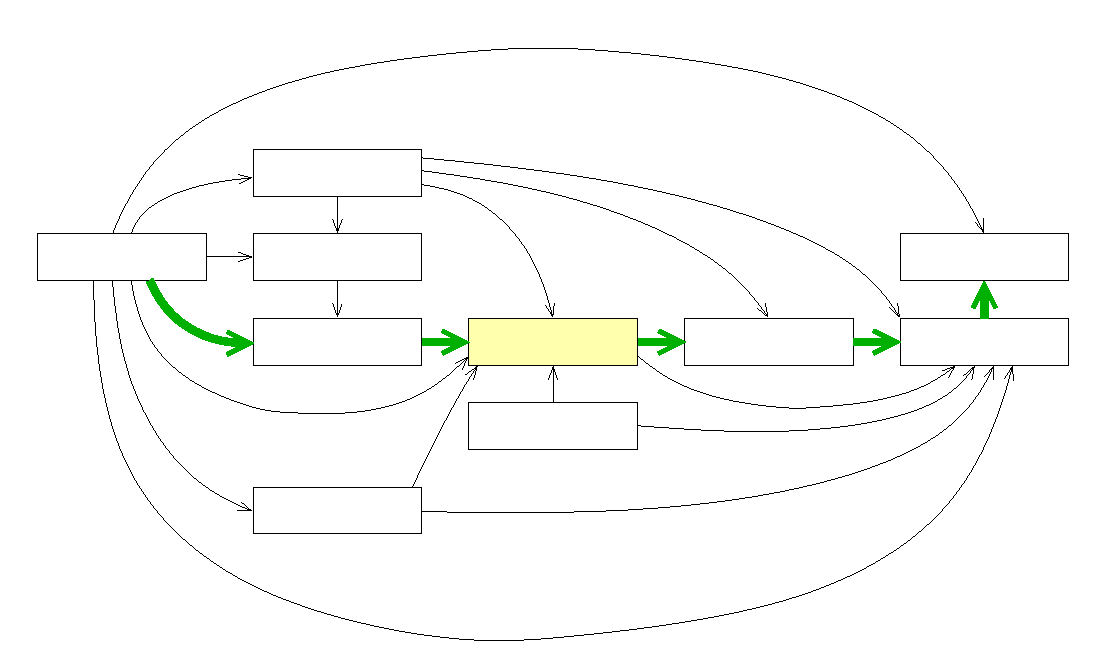
\includegraphics{getdp-struct-formulation}%
\end{picture}%
\setlength{\unitlength}{3947sp}%
%
\begingroup\makeatletter\ifx\SetFigFont\undefined%
\gdef\SetFigFont#1#2#3#4#5{%
  \reset@font\fontsize{#1}{#2pt}%
  \fontfamily{#3}\fontseries{#4}\fontshape{#5}%
  \selectfont}%
\fi\endgroup%
\begin{picture}(8274,4765)(439,-6402)
\put(1126,-3361){\makebox(0,0)[b]{\smash{\SetFigFont{10}{12.0}{\rmdefault}{\mddefault}{\updefault}{\color[rgb]{0,0,0}\code{Group}}%
}}}
\put(2851,-2686){\makebox(0,0)[b]{\smash{\SetFigFont{10}{12.0}{\rmdefault}{\mddefault}{\updefault}{\color[rgb]{0,0,0}\code{Function}}%
}}}
\put(2851,-3361){\makebox(0,0)[b]{\smash{\SetFigFont{10}{12.0}{\rmdefault}{\mddefault}{\updefault}{\color[rgb]{0,0,0}\code{Constraint}}%
}}}
\put(2851,-4036){\makebox(0,0)[b]{\smash{\SetFigFont{10}{12.0}{\rmdefault}{\mddefault}{\updefault}{\color[rgb]{0,0,0}\code{FunctionSpace}}%
}}}
\put(2851,-5386){\makebox(0,0)[b]{\smash{\SetFigFont{10}{12.0}{\rmdefault}{\mddefault}{\updefault}{\color[rgb]{0,0,0}\code{Jacobian}}%
}}}
\put(4576,-4711){\makebox(0,0)[b]{\smash{\SetFigFont{10}{12.0}{\rmdefault}{\mddefault}{\updefault}{\color[rgb]{0,0,0}\code{Integration}}%
}}}
\put(4576,-4036){\makebox(0,0)[b]{\smash{\SetFigFont{10}{12.0}{\rmdefault}{\mddefault}{\updefault}{\color[rgb]{0,0,0}\code{Formulation}}%
}}}
\put(6301,-4036){\makebox(0,0)[b]{\smash{\SetFigFont{10}{12.0}{\rmdefault}{\mddefault}{\updefault}{\color[rgb]{0,0,0}\code{Resolution}}%
}}}
\put(8026,-3361){\makebox(0,0)[b]{\smash{\SetFigFont{10}{12.0}{\rmdefault}{\mddefault}{\updefault}{\color[rgb]{0,0,0}\code{PostOperation}}%
}}}
\put(8026,-4036){\makebox(0,0)[b]{\smash{\SetFigFont{10}{12.0}{\rmdefault}{\mddefault}{\updefault}{\color[rgb]{0,0,0}\code{PostProcessing}}%
}}}
\end{picture}
}}

\chapter{\code{Formulation}: building equations}

\begin{slide}



Example:


\end{slide}

% ---------------------------------------------------------------------------

\background{7\semcm}{4.2\semcm}{\scalebox{0.3}{\begin{picture}(0,0)%
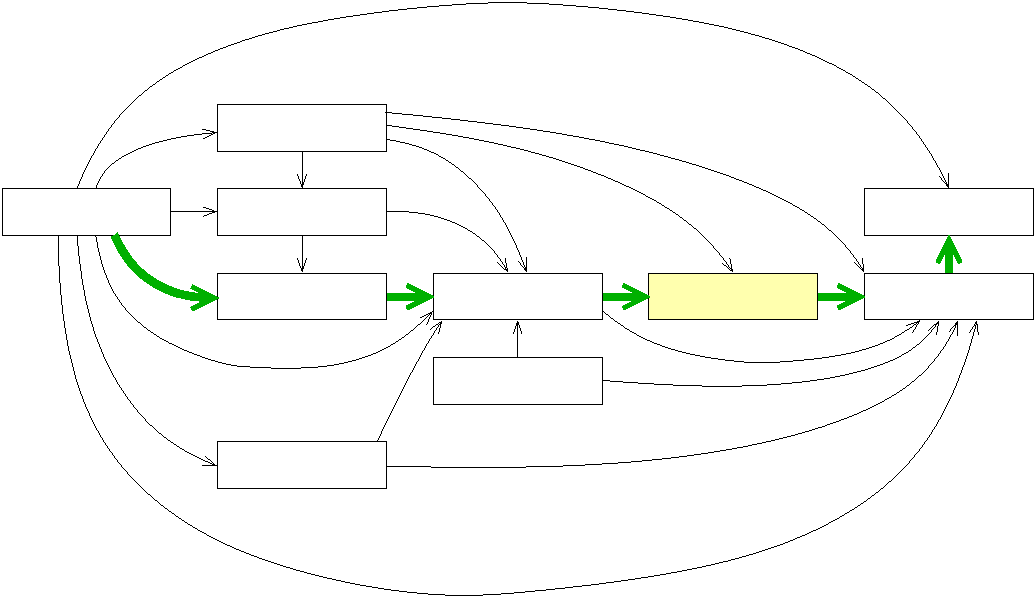
\includegraphics{getdp-struct-resolution}%
\end{picture}%
\setlength{\unitlength}{3947sp}%
%
\begingroup\makeatletter\ifx\SetFigFont\undefined%
\gdef\SetFigFont#1#2#3#4#5{%
  \reset@font\fontsize{#1}{#2pt}%
  \fontfamily{#3}\fontseries{#4}\fontshape{#5}%
  \selectfont}%
\fi\endgroup%
\begin{picture}(8552,4992)(300,-6402)
\put(1126,-3361){\makebox(0,0)[b]{\smash{\SetFigFont{10}{12.0}{\rmdefault}{\mddefault}{\updefault}{\color[rgb]{0,0,0}\code{Group}}%
}}}
\put(2851,-2686){\makebox(0,0)[b]{\smash{\SetFigFont{10}{12.0}{\rmdefault}{\mddefault}{\updefault}{\color[rgb]{0,0,0}\code{Function}}%
}}}
\put(2851,-3361){\makebox(0,0)[b]{\smash{\SetFigFont{10}{12.0}{\rmdefault}{\mddefault}{\updefault}{\color[rgb]{0,0,0}\code{Constraint}}%
}}}
\put(2851,-4036){\makebox(0,0)[b]{\smash{\SetFigFont{10}{12.0}{\rmdefault}{\mddefault}{\updefault}{\color[rgb]{0,0,0}\code{FunctionSpace}}%
}}}
\put(2851,-5386){\makebox(0,0)[b]{\smash{\SetFigFont{10}{12.0}{\rmdefault}{\mddefault}{\updefault}{\color[rgb]{0,0,0}\code{Jacobian}}%
}}}
\put(4576,-4711){\makebox(0,0)[b]{\smash{\SetFigFont{10}{12.0}{\rmdefault}{\mddefault}{\updefault}{\color[rgb]{0,0,0}\code{Integration}}%
}}}
\put(4576,-4036){\makebox(0,0)[b]{\smash{\SetFigFont{10}{12.0}{\rmdefault}{\mddefault}{\updefault}{\color[rgb]{0,0,0}\code{Formulation}}%
}}}
\put(6301,-4036){\makebox(0,0)[b]{\smash{\SetFigFont{10}{12.0}{\rmdefault}{\mddefault}{\updefault}{\color[rgb]{0,0,0}\code{Resolution}}%
}}}
\put(8026,-3361){\makebox(0,0)[b]{\smash{\SetFigFont{10}{12.0}{\rmdefault}{\mddefault}{\updefault}{\color[rgb]{0,0,0}\code{PostOperation}}%
}}}
\put(8026,-4036){\makebox(0,0)[b]{\smash{\SetFigFont{10}{12.0}{\rmdefault}{\mddefault}{\updefault}{\color[rgb]{0,0,0}\code{PostProcessing}}%
}}}
\end{picture}
}}

\chapter{\code{Resolution}: solving systems of equations}

\begin{slide}


Example:


\end{slide}

% ---------------------------------------------------------------------------

\background{7\semcm}{4.2\semcm}{\scalebox{0.3}{\begin{picture}(0,0)%
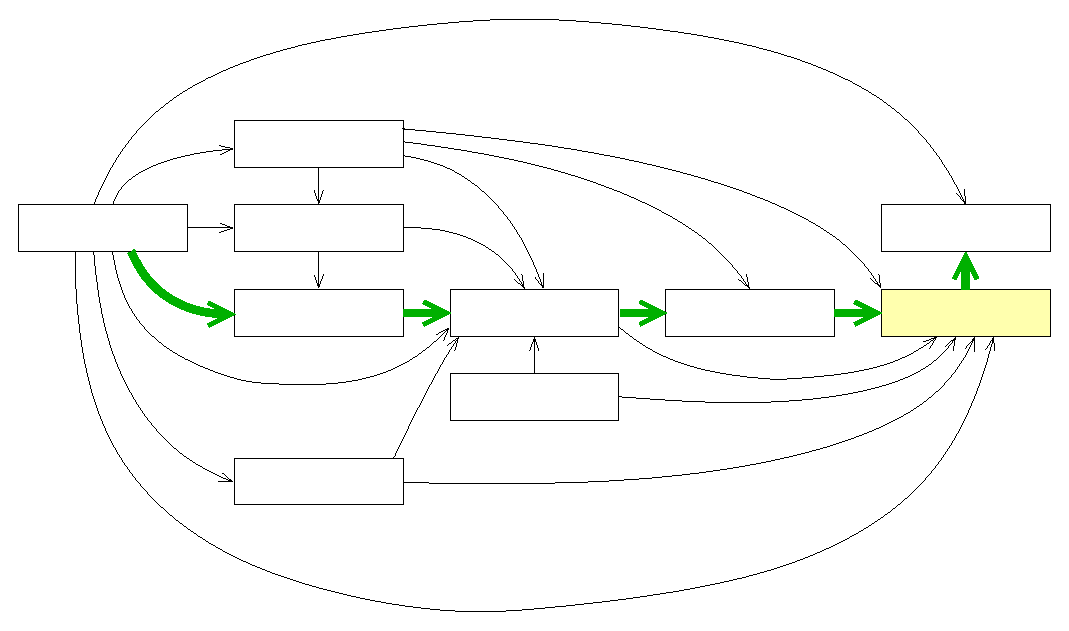
\includegraphics{getdp-struct-postprocessing}%
\end{picture}%
\setlength{\unitlength}{3947sp}%
%
\begingroup\makeatletter\ifx\SetFigFont\undefined%
\gdef\SetFigFont#1#2#3#4#5{%
  \reset@font\fontsize{#1}{#2pt}%
  \fontfamily{#3}\fontseries{#4}\fontshape{#5}%
  \selectfont}%
\fi\endgroup%
\begin{picture}(8274,4765)(439,-6402)
\put(1126,-3361){\makebox(0,0)[b]{\smash{\SetFigFont{10}{12.0}{\rmdefault}{\mddefault}{\updefault}{\color[rgb]{0,0,0}\code{Group}}%
}}}
\put(2851,-2686){\makebox(0,0)[b]{\smash{\SetFigFont{10}{12.0}{\rmdefault}{\mddefault}{\updefault}{\color[rgb]{0,0,0}\code{Function}}%
}}}
\put(2851,-3361){\makebox(0,0)[b]{\smash{\SetFigFont{10}{12.0}{\rmdefault}{\mddefault}{\updefault}{\color[rgb]{0,0,0}\code{Constraint}}%
}}}
\put(2851,-4036){\makebox(0,0)[b]{\smash{\SetFigFont{10}{12.0}{\rmdefault}{\mddefault}{\updefault}{\color[rgb]{0,0,0}\code{FunctionSpace}}%
}}}
\put(2851,-5386){\makebox(0,0)[b]{\smash{\SetFigFont{10}{12.0}{\rmdefault}{\mddefault}{\updefault}{\color[rgb]{0,0,0}\code{Jacobian}}%
}}}
\put(4576,-4711){\makebox(0,0)[b]{\smash{\SetFigFont{10}{12.0}{\rmdefault}{\mddefault}{\updefault}{\color[rgb]{0,0,0}\code{Integration}}%
}}}
\put(4576,-4036){\makebox(0,0)[b]{\smash{\SetFigFont{10}{12.0}{\rmdefault}{\mddefault}{\updefault}{\color[rgb]{0,0,0}\code{Formulation}}%
}}}
\put(6301,-4036){\makebox(0,0)[b]{\smash{\SetFigFont{10}{12.0}{\rmdefault}{\mddefault}{\updefault}{\color[rgb]{0,0,0}\code{Resolution}}%
}}}
\put(8026,-3361){\makebox(0,0)[b]{\smash{\SetFigFont{10}{12.0}{\rmdefault}{\mddefault}{\updefault}{\color[rgb]{0,0,0}\code{PostOperation}}%
}}}
\put(8026,-4036){\makebox(0,0)[b]{\smash{\SetFigFont{10}{12.0}{\rmdefault}{\mddefault}{\updefault}{\color[rgb]{0,0,0}\code{PostProcessing}}%
}}}
\end{picture}
}}

\chapter{\code{PostProcessing}: exploiting computational results}

\begin{slide}



Example:


\end{slide}

% ---------------------------------------------------------------------------

\background{7\semcm}{4.2\semcm}{\scalebox{0.3}{\begin{picture}(0,0)%
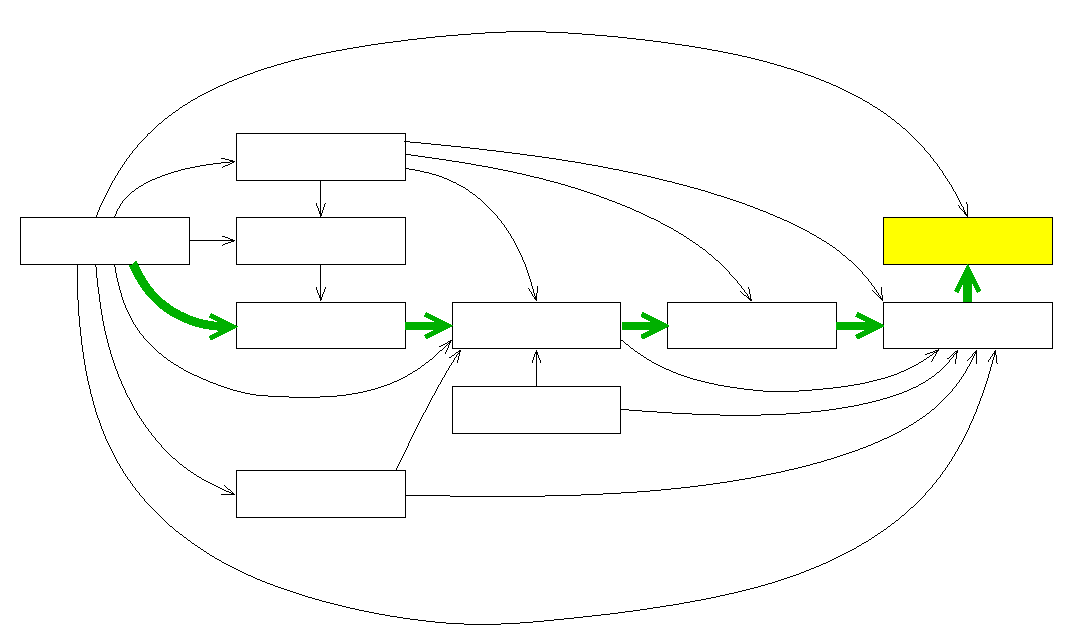
\includegraphics{getdp-struct-postoperation}%
\end{picture}%
\setlength{\unitlength}{3947sp}%
%
\begingroup\makeatletter\ifx\SetFigFont\undefined%
\gdef\SetFigFont#1#2#3#4#5{%
  \reset@font\fontsize{#1}{#2pt}%
  \fontfamily{#3}\fontseries{#4}\fontshape{#5}%
  \selectfont}%
\fi\endgroup%
\begin{picture}(8552,4992)(300,-6402)
\put(1126,-3361){\makebox(0,0)[b]{\smash{\SetFigFont{10}{12.0}{\rmdefault}{\mddefault}{\updefault}{\color[rgb]{0,0,0}\code{Group}}%
}}}
\put(2851,-2686){\makebox(0,0)[b]{\smash{\SetFigFont{10}{12.0}{\rmdefault}{\mddefault}{\updefault}{\color[rgb]{0,0,0}\code{Function}}%
}}}
\put(2851,-3361){\makebox(0,0)[b]{\smash{\SetFigFont{10}{12.0}{\rmdefault}{\mddefault}{\updefault}{\color[rgb]{0,0,0}\code{Constraint}}%
}}}
\put(2851,-4036){\makebox(0,0)[b]{\smash{\SetFigFont{10}{12.0}{\rmdefault}{\mddefault}{\updefault}{\color[rgb]{0,0,0}\code{FunctionSpace}}%
}}}
\put(2851,-5386){\makebox(0,0)[b]{\smash{\SetFigFont{10}{12.0}{\rmdefault}{\mddefault}{\updefault}{\color[rgb]{0,0,0}\code{Jacobian}}%
}}}
\put(4576,-4711){\makebox(0,0)[b]{\smash{\SetFigFont{10}{12.0}{\rmdefault}{\mddefault}{\updefault}{\color[rgb]{0,0,0}\code{Integration}}%
}}}
\put(4576,-4036){\makebox(0,0)[b]{\smash{\SetFigFont{10}{12.0}{\rmdefault}{\mddefault}{\updefault}{\color[rgb]{0,0,0}\code{Formulation}}%
}}}
\put(6301,-4036){\makebox(0,0)[b]{\smash{\SetFigFont{10}{12.0}{\rmdefault}{\mddefault}{\updefault}{\color[rgb]{0,0,0}\code{Resolution}}%
}}}
\put(8026,-3361){\makebox(0,0)[b]{\smash{\SetFigFont{10}{12.0}{\rmdefault}{\mddefault}{\updefault}{\color[rgb]{0,0,0}\code{PostOperation}}%
}}}
\put(8026,-4036){\makebox(0,0)[b]{\smash{\SetFigFont{10}{12.0}{\rmdefault}{\mddefault}{\updefault}{\color[rgb]{0,0,0}\code{PostProcessing}}%
}}}
\end{picture}
}}

\chapter{\code{PostOperation}: exporting results}

\begin{slide}



Example:


\end{slide}

% ---------------------------------------------------------------------------

\background{}{}{}


%% $Id: gmsh.tex,v 1.5 2001-06-13 16:00:29 geuzaine Exp $

\chapter{}

\begin{slide}

\slidepagestyle{reduced}

\begin{center}
\bigtitle{Gmsh --- Geometry, mesh, solver integration
and visualization}\\
\ifthenelse{\boolean{fulltitle}}{
\bigskip\bigskip
\begin{minipage}{0.5\textwidth}\center
\mediumtitle{Christophe Geuzaine}\\
\bigskip
\smalltitle{Dept. of Electrical Engineering}\\
\smalltitle{Montefiore Institute B28, Sart Tilman}\\
\smalltitle{University of Li�ge}\\
\smalltitle{B-4000 Li�ge (BELGIUM)}
\end{minipage}%
\begin{minipage}{0.5\textwidth}\center
\mediumtitle{Jean-Fran�ois Remacle}\\
\bigskip
\smalltitle{Scientific Computation Research Center}\\
\smalltitle{Rensselaer Polytechnic Insitute}\\
\smalltitle{CII 110 8th Street}\\
\smalltitle{Troy, New York 12180-3590 (USA)}
\end{minipage}}
\end{center}

\end{slide}

% ---------------------------------------------------------------------------
\part{Gmsh}
% ---------------------------------------------------------------------------

\chapter{Finite element methods in practice}

\begin{slide}

Four main steps:
\begin{slideitemize}
\item \emph{Geometry}: CAD sofware
\item \emph{Mesh}: structured or unstructed mesh generator
\item \emph{Solver}: GetDP :-)
\item \emph{Post-processing}: various visualization tools (2D and 3D)
\end{slideitemize}

Most of the time spent solving a problem is \emph{not} in the solver step!

\end{slide}

% ---------------------------------------------------------------------------

\background{7\semcm}{4.2\semcm}
           {\scalebox{0.3}{\input{fig/gmsh-geo.tex}}}

\chapter{Geometry description}

\begin{slide}

Constructive:


Parametric (scriptable):



\end{slide}

% ---------------------------------------------------------------------------

\background{7\semcm}{4.2\semcm}
           {\scalebox{0.3}{\input{fig/gmsh-mesh.tex}}}

\chapter{Mesh generation}

\begin{slide}

\begin{slideitemize}
\item \emph{Structured} (transfinite, elliptic, hyperbolic)
\item \emph{Unstructured} (Delaunay triangles/tetrahedra)
\begin{enumerate}
\item 
mesh of a box including the convex polygon/polyhedron resulting from
curves/surfaces discretization
\item
initial mesh by insertion of curves/surfaces nodes by the Bowyer algorithm
\item 
boundary restoration to force presence of all edges/faces
\item 
suppression of undesired triangles/tetrahedra
\item
new node insertions by the Bowyer algorithm until the characteristic size of
each simplex $\leq$ characteristic length field evaluated at the center of
its circumscribed circle/sphere.
\item
mesh post-processing and quality enforcement by node relocation and edge
swapping
\end{enumerate}
\end{slideitemize}

\end{slide}

% ---------------------------------------------------------------------------

\background{7\semcm}{4.2\semcm}
           {\scalebox{0.3}{\input{fig/gmsh-solver.tex}}}

\chapter{Solver integration}

\begin{slide}

\begin{minipage}{0.45\textwidth}
\emph{Batch}:
\begin{slideitemize}
\item Advanced users
\item No graphical overhead
\item Easily scriptable
\end{slideitemize}
$\rightarrow$ for heavy problems
\end{minipage}%
\begin{minipage}{0.1\textwidth}
vs.
\end{minipage}%
\begin{minipage}{0.45\textwidth}
\emph{Interactive}:
\begin{slideitemize}
\item Smoother learning curve
\item Better integration
\item Faster for testing
\end{slideitemize}
$\rightarrow$ for testing/learning
\end{minipage}%

\end{slide}

\begin{slide}

Example: integration of GetDP into higher level toolboxes (visualization,
optimization, etc.):
\begin{slideitemize}
\item \emph{High level}: Commercial applications (Matlab, Mathematica, ...),
shell scripts (bash, Perl, Python, ...), other programming languages (C,
C++, ...) 

$\rightarrow$ \emph{system calls}
\item \emph{Medium level}: Home-grown applications (Gmsh, ...), shell scripts
(Perl, Python, ...), other programming languages (C, C++, ...) 

$\rightarrow$ \emph{sockets}
\item \emph{Low level}: programming languages (C, C++, ...) 

$\rightarrow$ \emph{source code}
\end{slideitemize}

\end{slide}

% ---------------------------------------------------------------------------

\background{7\semcm}{4.2\semcm}
           {\scalebox{0.3}{\input{fig/gmsh-postpro.tex}}}

\chapter{Post-processing}

\begin{slide}

Scriptable:

Modular:


\end{slide}

% ---------------------------------------------------------------------------



% ---------------------------------------------------------------------------
\part{Collaboration}
% ---------------------------------------------------------------------------

\chapter{Possible collaboration topics}

\begin{slide}

\begin{slideitemize}
\item Error estimation
\item Optimization
\end{slideitemize}

\end{slide}

% ---------------------------------------------------------------------------
\part{Conclusion}
% ---------------------------------------------------------------------------

\end{document}

